\section{Preliminaries}
\subsection{Notation}
\label{sec:notations}

\Cref{tab:notation} summarizes the notation we use throughout this paper.
We use bold uppercase letters for matrices and lowercase letters for vectors.
For matrix rows and columns, we employ MATLAB notation, i.e., $\AA(i, :)$ and $\AA(:, j)$ refer to the $i$th row and the $j$th column of $\AA$.
We use subscripts to refer to sub-blocks of matrices.
For example, $\AA_ij$ refers to the sub-block $(i, j)$ of $\AA$ in a 2D partition.
We use $m$ and $n$ to denote the numbers of rows and columns of $\AA$, respectively, and assume without loss of generality $m\geq n$ throughout.

\begin{table}%[htdp]
\begin{center}
\begin{tabular}{|l|l|}
\hline
$\AA$ & Input matrix \\
$\WW$ & Left low rank factor \\
$\HH$ & Right low rank factor \\
$m$ & Number of rows of input matrix \\
$n$ & Number of columns of input matrix \\
$k$ & Low rank \\
$P$ & Number of parallel processes \\
$P_r$ & Number of rows in processor grid \\
$P_c$ & Number of columns in processor grid \\
$\Ip$,$\Jp$ & Set of rows/columns of of $\Wm$/$\Hm$ owned by process $p$  \\
$\Fp$,$\Gp$ & Set of unique row and column indices of $\Amp$ \\
$\Amp$ & Submatrix of $\Am$ owned by process p \\
$\Wm(\Ip,:)$ & Owned rows of initial $\Wm$ by process p \\
$\Hm(:,\Jp)$ & Owned columns of initial $\Hm$ by process p\\

\hline
\end{tabular}
\end{center}
\caption{Notation}
\label{tab:notation}
\end{table}%


\subsection{Communication model}
\label{sec:comm-model}

To analyze our algorithms, we use the $\alpha$-$\beta$-$\gamma$ model of distributed-memory parallel computation.
In this model, interprocessor communication occurs in the form of messages sent between two processors across a bidirectional link (we assume a fully connected network).
We model the cost of a message of size $n$ words as $\alpha+n\beta$, where $\alpha$ is the per-message latency cost and $\beta$ is the per-word bandwidth cost.
Each processor can compute floating point operations (flops) on data that resides in its local memory; $\gamma$ is the per-flop computation cost.
With this communication model, we can predict the performance of an algorithm in terms of the number of flops it performs as well as the number of words and messages it communicates.
For simplicity, we will ignore the possibilities of overlapping computation with communication in our analysis.
For more details on the $\alpha$-$\beta$-$\gamma$ model, see \cite{TRG05,CH+07}. Since one of the major objective of this paper is comparing the communications strategies between different distribution strategies -- point-to-point communication for $NNZ-PART$ and the collective communications for $2D$. For the collective communication for $2D$, we are observing the same communication model of the \mpifaun algorithm \cite{KBP16, KBP16MPIFAUN}. We present the communication model for P2P here. 

\subsection{Point-to-Point Communication}

\todo{\oguz{fill the point to point communication on pacoss}}

%\subsection{MPI collectives}
%\label{sec:collectives}
%
%Point-to-point messages can be organized into collective communication operations that involve more than two processors.
%MPI provides an interface to the most commonly used collectives like broadcast, reduce, and gather, as the algorithms for these collectives can be optimized for particular network topologies and processor characteristics.
%The baseline algorithms $MPIFAUN$ use the all-gather, reduce-scatter, and all-reduce collectives and so we review them here, along with their costs.
%%Our analysis assumes optimal collective algorithms are used (see \cite{TRG05,CH+07}), though our implementation relies on the underlying MPI implementation.
%
%At the start of an all-gather collective, each of $p$ processors owns data of size $n/p$.
%After the all-gather, each processor owns a copy of the entire data of size $n$.
%The cost of an all-gather is $\alpha\cdot \log p + \beta \cdot \frac{p-1}{p}n$.
%%
%At the start of a reduce-scatter collective, each processor owns data of size $n$.
%After the reduce-scatter, each processor owns a subset of the sum over all data, which is of size $n/p$.
%(Note that the reduction can be computed with other associative operators besides addition.)
%The cost of an reduce-scatter is $\alpha\cdot \log p + (\beta+\gamma) \cdot \frac{p-1}{p}n$.
%%
%At the start of an all-reduce collective, each processor owns data of size $n$.
%After the all-reduce, each processor owns a copy of the sum over all data, which is also of size $n$.
%The cost of an all-reduce is $2\alpha\cdot \log p + (2\beta+\gamma) \cdot \frac{p-1}{p}n$.
%%
%Note that the costs of each of the collectives are zero when $p=1$.

\section{Sparse Non-negative Matrix Factorization}
\label{sec:sparsenmf}

%We are extending the $AUNMF$ algorithm in \mpifaun framework \cite{KBP16MPIFAUN, KBP16} for implementing different NMF algorithms to add support for sparse input matrix.
The Alternating-Updating NMF algorithms are those that alternate between updating one of $\WW$ and $\HH$ using the given input matrix $\AA$ and other 'fixed' factor - $\HH$ for updating $\WW$ or $\WW$ for updating $\HH$.
This update is performed using the Gram matrix associated with the fixed factor matrix, and the product of the input matrix $\AA$ with the fixed factor matrix.
We show the structure of the framework in \cref{alg:aunmf}. 

%Different algorithms determine $\WW$ and $\HH$ by partitioning these matrices in different ways and can be explained under Block Coordinate Descent (BCD) framework. 
%Generally, these matrices are determined as (a) 2-Blocks of entire matrix $\WW$ and $\HH$; (b) $2k$ blocks such as $[\ww^1, \ww^2, \cdots , \ww^m] \in \Rnplus{k}$ and $[\hh_1^T, \hh_2^T, \cdots , \hh_n^T] \in \Rnplus{k}$ \footnote{For convenience, $\M{x}^i$ is the $i$th column vector of matrix $\M{X}$ and $\M{x}_i$ is the $i$th row vector} and (c) $(m+n)k$ scalar blocks of $w_{ik} \in \WW$ and $h_{kj} \in \HH$. 

\begin{algorithm}
\caption{$[\WW,\HH] = \text{AU-NMF}(A,k)$}
\label{alg:aunmf}
\begin{algorithmic}[1]
\REQUIRE $\AA$ is an $m\times n$ matrix, $k$ is rank of approximation
\STATE Initialize $\HH$ with a non-negative matrix in $\Rn{n\times k}_+$.
\WHILE{stopping criteria not satisfied} \label{algo:nmfloop}
  \STATE Update $\WW$ using $\HH \HH^T$ and $\AA \HH^T$ \label{line:aunmf-w}
  %\STATE Update $\WW$ as $\Argmin{\tilde \WW\geq 0}\NormBr{\AA-\tilde\WW\HH}_F$
  %\STATE Update all blocks defined over $\WW$
  \label{line:aunmf:W}
  \STATE Update $\HH$ using $\WW^T\WW$ and $\WW^T \AA$ \label{line:aunmf-h}
  %\STATE Update $\HH$ as $\Argmin{\tilde\HH\geq 0}\NormBr{\AA-\WW\tilde\HH}_F$
  %\STATE Update all blocks defined over $\HH$
  \label{line:aunmf:H}
\ENDWHILE
\end{algorithmic}
\end{algorithm}

After computing the Gram matrix and the multiplication of $\AA$ with the fixed factor matrix, the specifics of the update at \cref{line:aunmf:W,line:aunmf:H} depend on the NMF algorithm, and we refer to the computation associated with these lines as the Local Update Computations (\LUC).
%Because these computations are performed locally, we use a function $F(m,n,k)$ to denote the number of flops required for each algorithm's \LUC\ (and we do not consider communication costs).

We note that AU-NMF is very similar to a two-block, block coordinate descent (BCD) framework as explained by Bertsekas \cite{bertsekas1999nonlinear}.
The BCD framework expresses solving optimization variables in complex non-linear optimization problem as one block at a time, while keeping the others fixed. In NMF,  the two blocks are
the unknown factors $\WW$ and $\HH$, 
and we \emph{solve} the following subproblems,
which have a unique solution for a full rank $\HH$ and $\WW$: 
\SplitN{\label{eqn:two block}} {
\WW &\leftarrow \Argmin{\tilde \WW\geq 0}\NormBr{\AA-\tilde\WW\HH}_F +  \phi (\tilde \WW) + \psi (\HH),\\
\HH &\leftarrow  \Argmin{\tilde\HH\geq 0}\NormBr{\AA-\WW\tilde\HH}_F + \phi (\WW) + \psi (\tilde \HH).
}

Since each subproblem involves non-negative least squares,
this two-block BCD method is also called
the Alternating Non-negative Least Squares (ANLS) method \cite{kim2013nonnegative}.
Block Principal Pivoting (\BPP) is one algorithm that solves these NLS subproblems.
In the context of the AU-NMF algorithm,
 an ANLS method {\em maximally} reduces 
the overall NMF objective function value 
by finding the optimal solution for
 given $\HH$ and $\WW$ in \cref{line:aunmf:W,line:aunmf:H}, respectively.  

%There are other popular NMF algorithms 
%that update the factor matrices alternatively
%without maximally reducing the objective function value each time,
%in the same sense as in ANLS. 
From time to time, these updates do not necessarily solve each of the subproblems \eqref{eqn:two block} to optimality but simply improve the overall objective function \eqref{eqn:original NMF}.  
such as Multiplicative Update (\MU) \cite{seung2001algorithms} and Hierarchical Alternating Least Squares (\HALS) \cite{cichocki2009nonnegative}.

The convergence properties of these different NMF algorithms are discussed in detail by Kim, He and Park \cite{kim2013nonnegative}.
While we focus only on the \MU algorithms in this paper, we highlight that our algorithm is not restricted to this, and is seamlessly extensible to other NMF algorithms as well, including \HALS, \BPP, Alternating Direction Method of Multipliers (\textbf{ADMM}) \cite{SF14}, and Nesterov-based methods \cite{GTLY12}. 

%Here, we have explained the update equations of the NMF algorithms ANLS/BPP, HALS and MU. In all these three algorithms, the update equations uses $\AA\HH^T$ and $\HH\HH^T$ for line \ref{line:anls:W} and $\WW^T\AA$ and $\WW^T\WW$ for line \ref{line:anls:H}.

%As in the Figure \ref{fig:2blocks}, the ANLS/BPP \cite{kim2011fast} is an example of 2-Blocks BCD that determines $\WW$ and $\HH$ as matrix blocks by solving 
%the following equations using active set method iteratively until a stopping criteria is satisfied: 


%\begin{figure*}
%\subfloat[][ANLS/BPP 2-Blocks BCD] {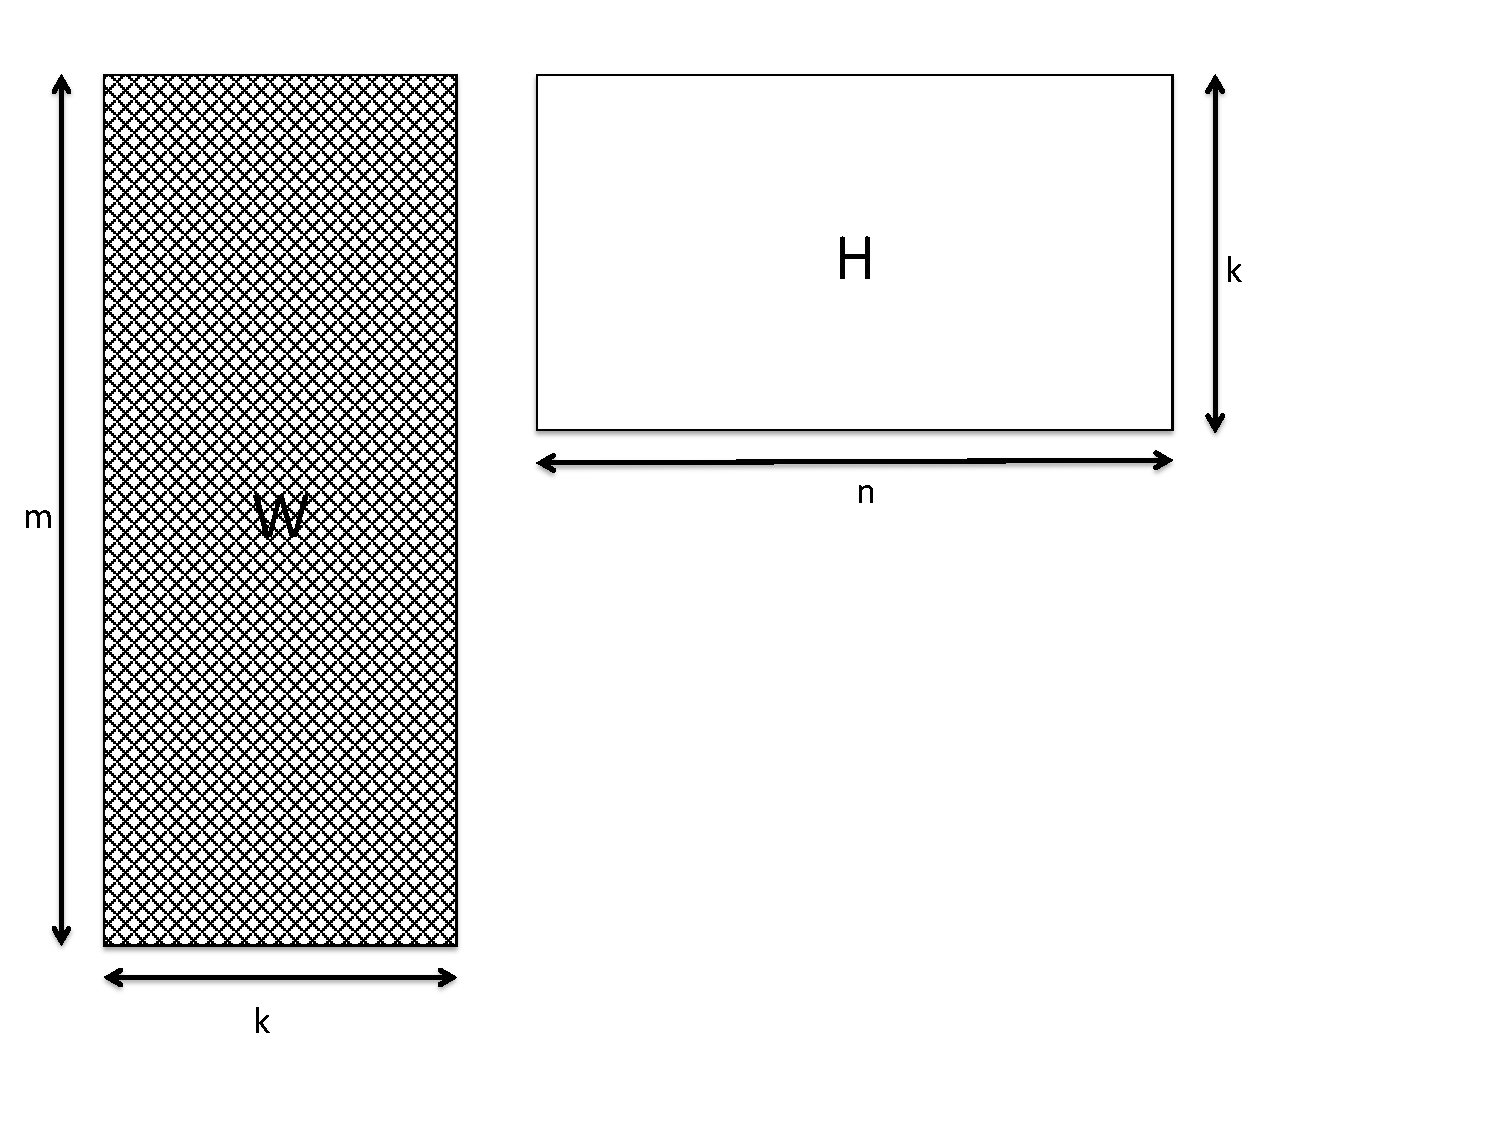
\includegraphics[height=1.5in, width=2.5in]{fig/bcd2blocks}\label{fig:2blocks}}
%\subfloat[][HALS 2k-Blocks BCD] {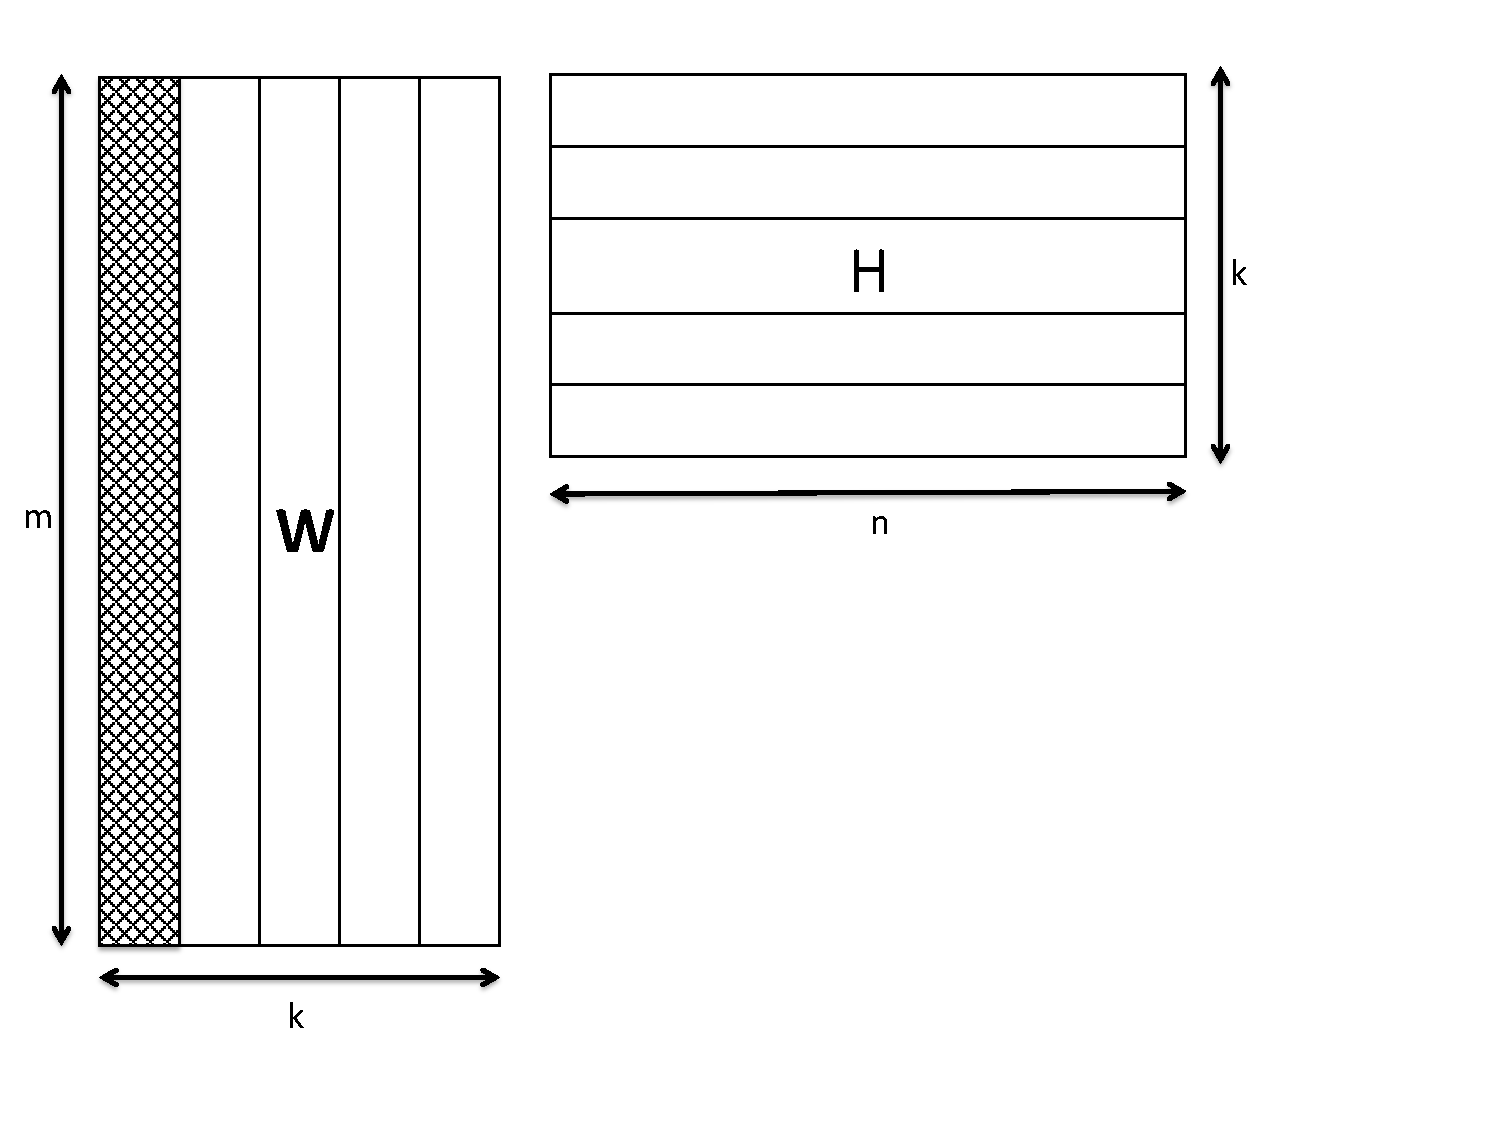
\includegraphics[height=1.5in, width=2.5in]{fig/bcd2kblocks}\label{fig:2kblocks}}
%\subfloat[][MU (m+n)k Scalar Blocks BCD] {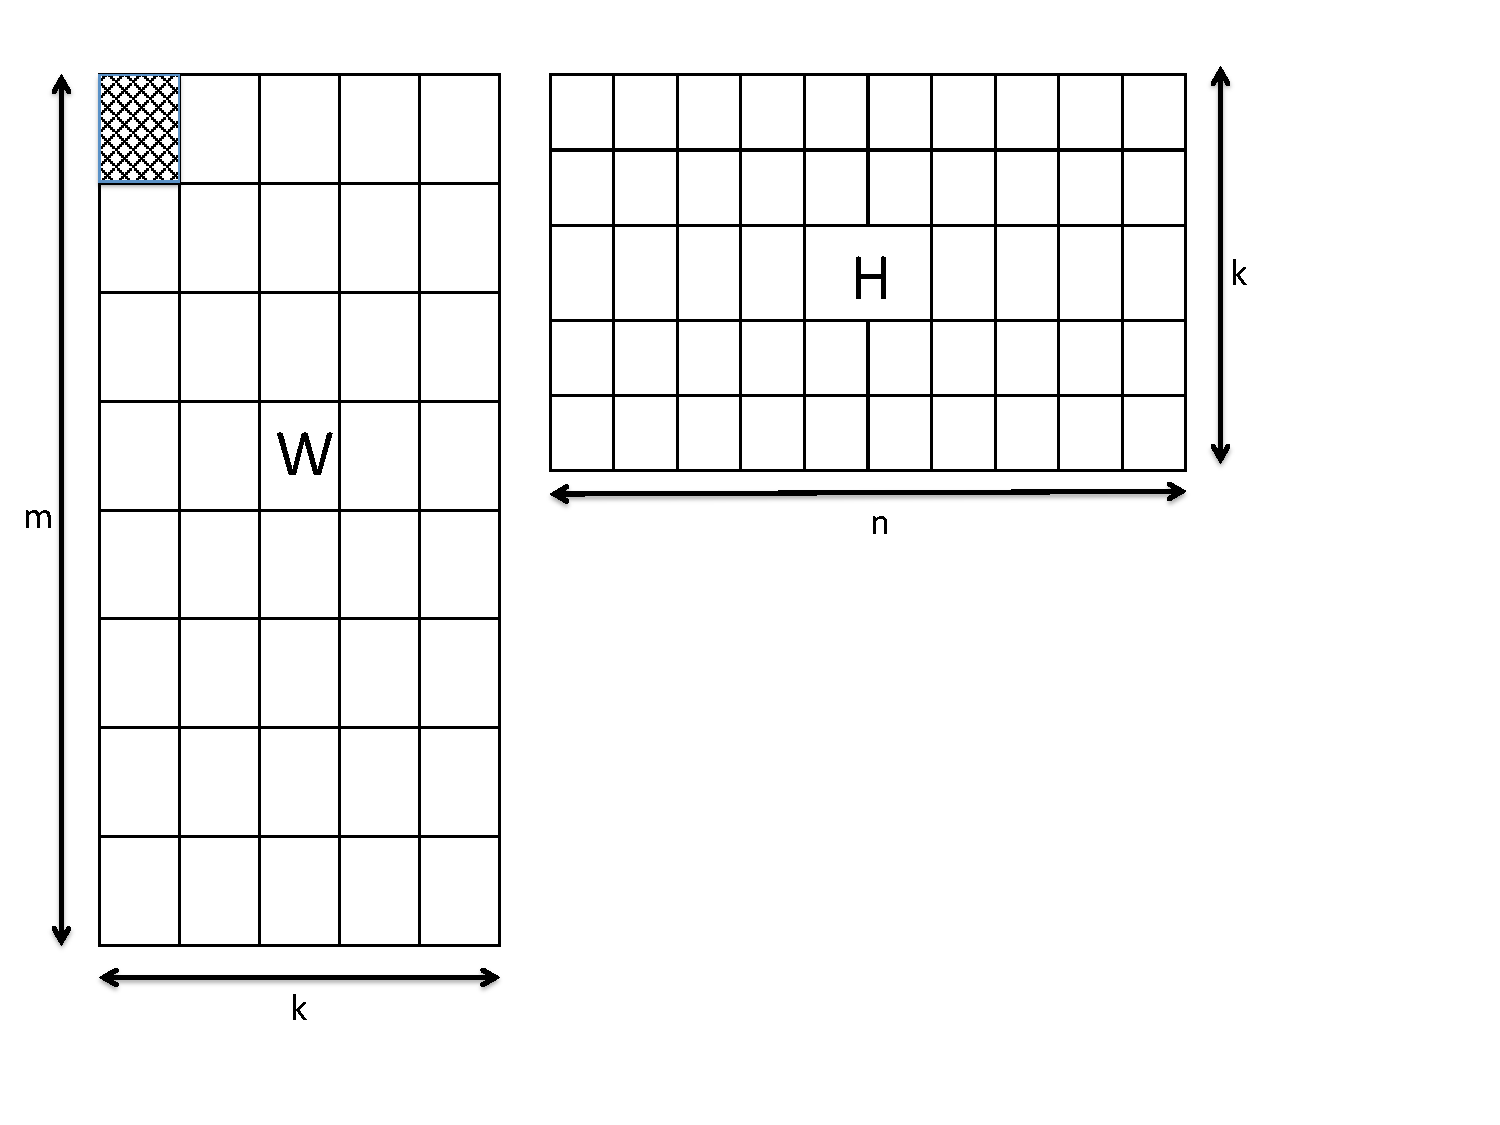
\includegraphics[height=1.5in, width=2.5in]{fig/bcdscalarblocks}\label{fig:bcdscalarblocks}}
%\end{figure*}

\subsection{Multiplicative Update (\MU)}
\label{sec:sparsenmfmu}

In this paper, we are considering $\ell_2$ regularization on the $\WW$ matrix and $\ell_1$ regularization on the $\HH$ matrix to address the sparsity of the input matrix. Hence, the NMF problem becomes
 \SplitN{\label{eqn:original NMF}}{
\min_{\WW \geq 0,\HH \geq 0} & \|\AA-\WW\HH\|_F + \alpha (\| \WW \|)_F^2 + \beta \sum_{i=1}^n \| \hh_{i} \|_1^2.
}

The values $\alpha$ and $\beta$ were fixed for the experiments. 
In the case of \MU\ \cite{seung2001algorithms}, individual entries of $\WW$ and $\HH$ are updated with all other entries fixed.
In this case, the update rules are 
\SplitN{\label{eqn:muupdate}} {
w_{ij} &\leftarrow w_{ij} \frac{(\AA \HH^T)_{ij}}{(\WW (\HH \HH^T+ 2\beta \mathbf{1}_k))_{ij}}, \text{ and }\\
h_{ij} &\leftarrow  h_{ij} \frac{(\WW^T \AA)_{ij}}{((\WW^T \WW+ 2\alpha\mathbf{I}_k) \HH)_{ij}}.
} 
where $\mathbf{1}_k$ is a matrix of $k \times k$ with all one's and $\mathbf{I}_k$ is an identity matrix of size $k \times k$. 

After computing the Gram matrices $\HH\HH^T$ and $\WW^T \WW$, adding the appropriate regularizers and the products $\AA\HH^T$ and $\WW^T\AA$, the extra cost of computing $\WW (\HH \HH^T+ 2\beta \mathbf{1}_k)$ and $(\WW^T \WW+ 2\alpha\mathbf{I}_k)$ is $F(m,n,k)=2(m+n)k^2$ flops to perform updates for all entries of $\WW$ and $\HH$, as the other elementwise operations affect only lower-order terms.
The details about using AU-NMF in \cref{alg:aunmf} for other algorithms \HALS\ and \BPP\ are explained in~\cite{KBP16,KBP16MPIFAUN}. 

The above update equation \cref{eqn:muupdate} can be easily parallelized using the \cref{alg:distnmf}. 

%To begin with let us consider the 1D row distribution of the the matrix $\AA$, where each process hold $\frac{m}{p} \times n$ represented as $\AA^i$ and the entire $\HH \in \Rnplus{k \times n}$. Every  $\AA^i\HH^T \in $   

It is important to observe that the update function of $\WW$ is element-wise normalization of the sparse matrix-dense matrix multiplication $\AA \HH^T$ with the denominator. Given that if all the processes owns the $k \times k$ gram of the factor matrix $\HH$, computing the entire denominator $(\WW (\HH \HH^T+ 2\beta \mathbf{1}_k))$ is does not require any communication, hence can be done locally.
%We can see that the \cref{line:hmgr} and \cref{line:foldw} offers the local processes' $\AA \HH^T$.
One can argue that the same holds for updating $\HH$ as well.
Therefore, for row and column index sets $\Ip$ and $\Jp$, one can update these rows of the factor matrices as follows:

\SplitN{\label{eqn:muupdate}} {
\Wm(\Ip, :) &\leftarrow \Wm(\Ip, :) \circledast (\Wmt(\Ip, :)) \oslash (\Wm(\Ip, :) (\Hmgr+ 2\beta \mathbf{1}_k)), \text{ and }\\
\Hm(\Jp, :) &\leftarrow  \Hm(\Jp, :) \circledast (\Hmt(\Jp, :) \oslash (\Wmgr+ 2\alpha\mathbf{I}_k) \Hm(\Jp, :)).
}
where $\circledast$ and $\oslash$ correspond to element-wise multiplication and division of matrices or vectors.
This scheme provides row-wise parallelism in NNLS computation.
\HALS\ and \BPP can similarly be expressed in this row-parallel form.

%\todo{\ramki{ramki can you explain that we can row-wise parallelize this computation? Specificaly, we need to say that $\Wm(I, :)$ can be updated using $\Hm \Hm^T$ and the submatrix $[\Am \Hm] (I, :)$}}

%Apart from the proposed \distspnmf Algorithm \ref{alg:distnmf}, we have to extend the \mpifaun framework for $2D$ partition strategy in the following directions (a) Additional sparse regularization which otherwise will result in numerical in-stability for large high-dimensional sparse matrices (b) The intermediate memory requirement for \mpifaun restricts its ability to handle sparse matrices of few hundred millions and more in smaller processor and we have to extend blocking support on the low rank side. 

%\input{hypergraph}
